%%%%%%%%%%%%%%%%%%%%%%%%%%%%%%%%%%%%%%%%
% Class options                        %
%%%%%%%%%%%%%%%%%%%%%%%%%%%%%%%%%%%%%%%%
% Orientation:                         %
% portrait (default), landscape        %
%                                      %
% Paper size:                          %
% a0paper (default), a1paper, a2paper, %
% a3paper, a4paper, a5paper, a6paper   %
%                                      %
% Language:                            %
% english (default), norsk             %
%%%%%%%%%%%%%%%%%%%%%%%%%%%%%%%%%%%%%%%%
% \documentclass[landscape]{uioposter}
\documentclass[portrait]{uioposter}


\usepackage{lipsum}                                % Dummy text
\usepackage[figwidth = 0.98\linewidth]{todonotes}  % Dummy image (and more!)
\usepackage[absolute, overlay]{textpos}            % Figure placement
\setlength{\TPHorizModule}{\paperwidth}
\setlength{\TPVertModule}{\paperheight}

\usepackage[backend=biber,sorting=none,hyperref=true,style=numeric,isbn=false,doi=false,eprint=false,url=false,]{biblatex}
\addbibresource{poster_bib.bib}
\renewcommand*{\bibfont}{\tiny}




\title{CMS RPC Upgrade Program}
\author
{%
    Felipe Silva, on behalf of the CMS Collaboration
    % \and
    % Second Author%\inst{2}
    % \and
    % Third Author%\inst{1}
}
%% Optional:
\institute
{
   Rio de Janeiro State University - Email: felipe.silva@cern.ch
%    \and
%    \inst{2} Department of Informatics
}
% Or:
% \institute{Contact information}


%% Remove footline:
% \setbeamertemplate{footline}{}
  

\begin{document}
\begin{frame}


    % \vskip-2cm
    \begin{block}{Abstract}
        \vskip-1.5cm
        The LHC will be upgraded in several phases that will allow significant expansion of its physics program. The luminosity of the accelerator is expected to exceed $5 \times 10^{34} cm^{-2}s^{-1}$.  In order to sustain the harsher conditions and to help maintaining good trigger efficiency and performance the Resistive Plate Chambers (RPC) system of the CMS experiment will be upgraded. The present RPC system would continue to operate, and it would be upgraded with new Link Boards system. In addition, the coverage of the RPC system would be increased up to pseudo rapidity of 2.4 by installing a new generation of improved RPCs (iRPCs). Their design and configuration are optimized to sustain higher rates and hence to survive the harsh background condition during HL-LHC operation. The iRPC are equipped with newly developed electronics designed to read out the detectors from both sides, allowing in this way a good spatial resolution along the strips O(cm). The status of the upgrade project is presented.
    \end{block}

\begin{columns}[onlytextwidth]


\begin{column}{\textwidth/2 - 1cm}

    \vskip-2cm
    \begin{block}{CMS RPC Upgrade}
        \vskip-1.5cm
        

Figure~\ref{cms_muon_upgrade} presents a quadrant of the CMS Muon system, showing DT chambers (yellow), RPCs (light blue), and CSCs (green). The locations of new forward muon detectors for the HL-LHC project are indicated in red for Gas Electron Multiplier (GEM) stations (ME0, GE1/1, and GE2/1) and violet for improved RPC stations (RE3/1 and RE4/1).

\begin{wrapfigure}{r}{0.5\textwidth}
    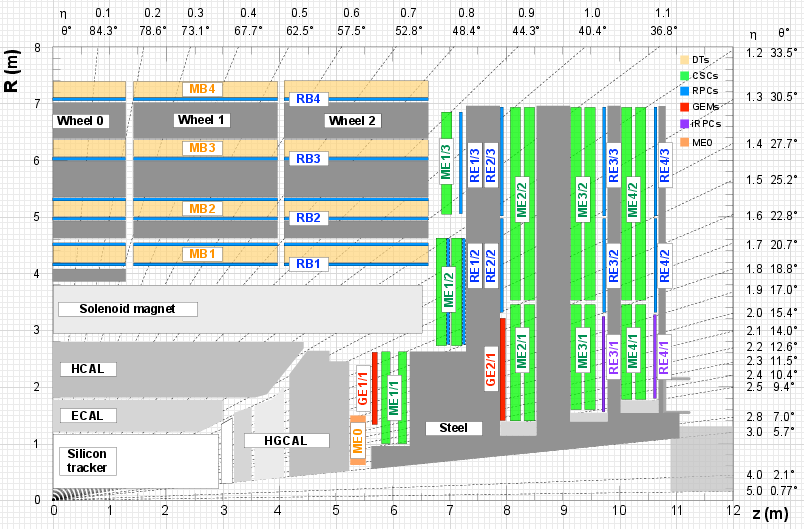
\includegraphics[width=0.5\textwidth]{uioposter-images/cms_muon}
    \caption{CMS Muon system for the Phase-2 Upgrade.}
    \label{cms_muon_upgrade}
\end{wrapfigure}

Bla bla bla... Bla bla bla... Bla bla bla... Bla bla bla... Bla bla bla... Bla bla bla... Bla bla bla... Bla bla bla... Bla bla bla... Bla bla bla... Bla bla bla... Bla bla bla... Bla bla bla... Bla bla bla... Bla bla bla... Bla bla bla... Bla bla bla... Bla bla bla... Bla bla bla... Bla bla bla... Bla bla bla... Bla bla bla... Bla bla bla... Bla bla bla... Bla bla bla... Bla bla bla... Bla bla bla... Bla bla bla... Bla bla bla... Bla bla bla... Bla bla bla... Bla bla bla... Bla bla bla... Bla bla bla... Bla bla bla... Bla bla bla... 

Bla bla bla... Bla bla bla... Bla bla bla... Bla bla bla... Bla bla bla... Bla bla bla... Bla bla bla... Bla bla bla... Bla bla bla... Bla bla bla... Bla bla bla... Bla bla bla... Bla bla bla... Bla bla bla... Bla bla bla... Bla bla bla... Bla bla bla... Bla bla bla... Bla bla bla... Bla bla bla... Bla bla bla... Bla bla bla... Bla bla bla... Bla bla bla... Bla bla bla... Bla bla bla... Bla bla bla... Bla bla bla... Bla bla bla... Bla bla bla... Bla bla bla... Bla bla bla... Bla bla bla... Bla bla bla... Bla bla bla... Bla bla bla... 
    \end{block}

    \vskip-2cm
    \begin{block}{Link System}
        \vskip-1.5cm
        % Bla bla bla ...

% % \begin{figure}
%     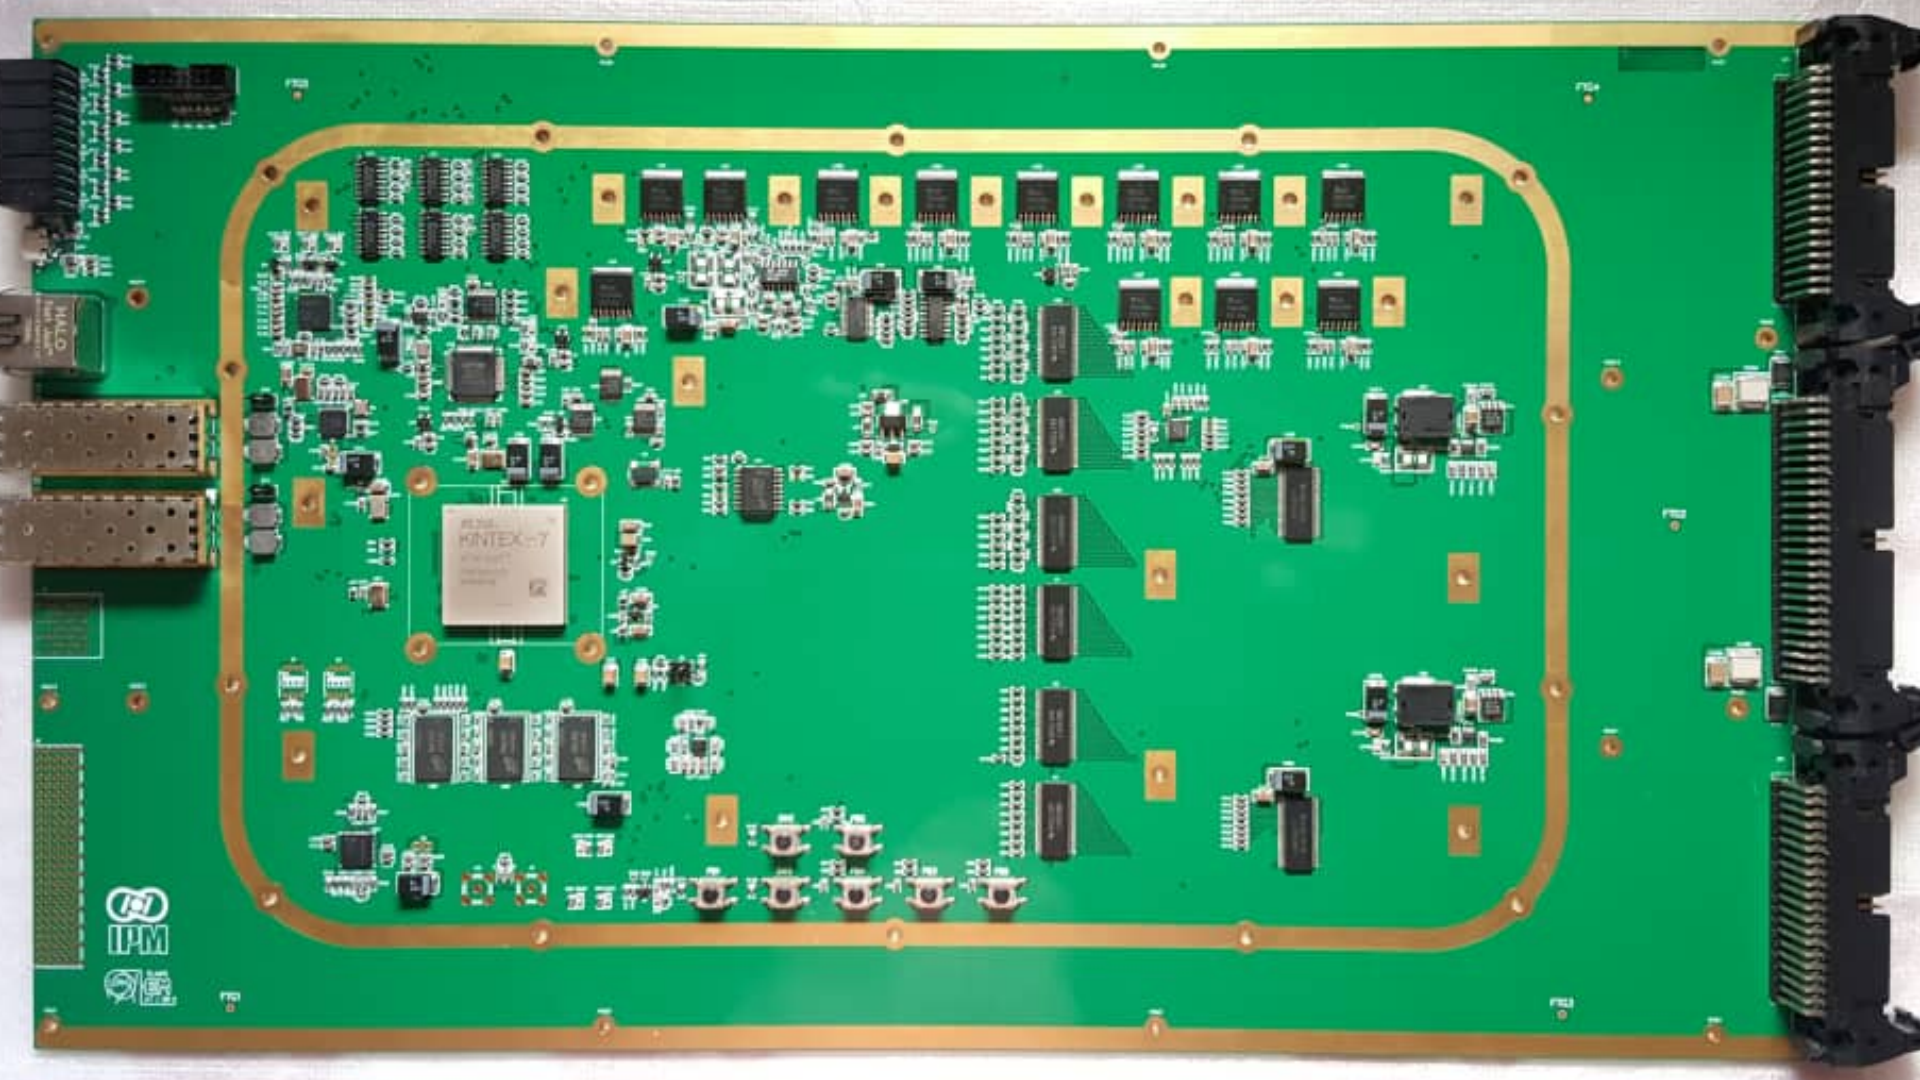
\includegraphics[width=1\textwidth]{uioposter-images/link_system_board}
%     % \caption{\footnotesize A quadrant of the CMS Muon Spectrometer, showing DT chambers (yellow), RPCs (light blue), and CSCs (green). The locations of new forward muon detectors for the HL-LHC project are contained within the dashed box and indicated in red for Gas Electron Multiplier (GEM) stations (ME0, GE1/1, and GE2/1) and violet for improved RPC stations (RE3/1 and RE4/1).}
% %     \label{cms_muon_upgrade}
% % \end{figure}

% Bla bla bla ...



In the CMS experiment, the RPC chambers are readout, controlled and monitored through the Link System, which consists of 1592 electronics boards, divided in two kinds, known as the Link boards (LBs) and Control Boards (CBs), LBs can work as Master LB or Slave LB.  

% Details of the CMS RPC readout and control are shown in Figure~\ref{rpc_phase2_readout}.

\begin{wrapfigure}[6]{r}{0.5\textwidth}
    % \hskip1cm
    \caption{\footnotesize A RPC Link Board prototype for Phase-2 Upgrade.}
    \label{link_system}.
    % \hfill
    % \center
    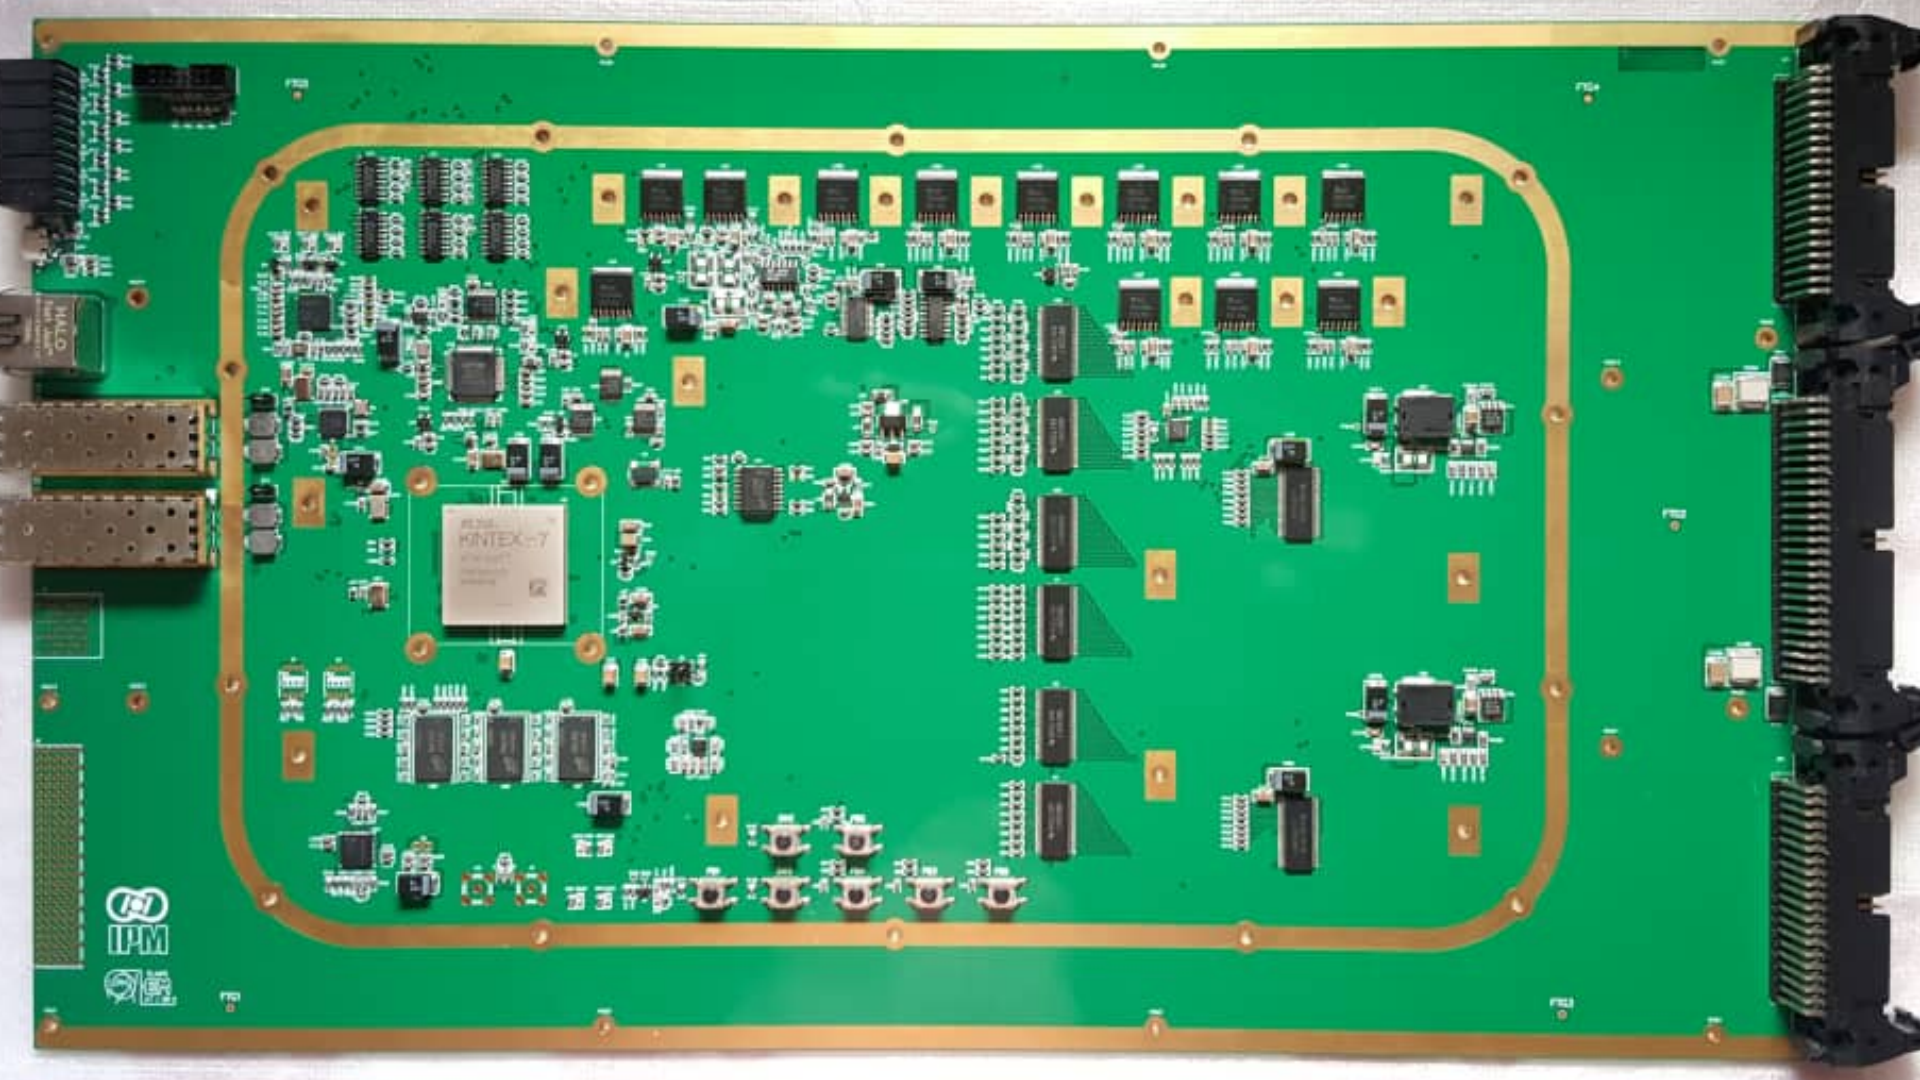
\includegraphics[width=0.49\textwidth]{uioposter-images/link_system_board.png}
\end{wrapfigure}

% The HL-LHC high rates will required an increase of the available TX bandwidth and readout time resolution. 

The new link system is being developed around the use of modern components and FPGAs (Field Programmable Gate Array), following a radiation hard design. 

\begin{tcolorbox}[colback=gray!5,colframe=gray!40!black]
    \textbf{The data transmission rate between the new Link system and RPC back-end electronics increases to 10.24 Gbps and resolution of the Muon hit time improves to 1.5 ns.}
\end{tcolorbox}

% \textbf{}

\hfill

This is achieved by \textbf{(1) the use GTX transceivers of the FPGA}, plus preprocessing of data and (2) implementing a high resolution \textbf{96-channel Time-to-Digital Converter (TDC) in the link board FPGA}. Each TDC channel comprised of 16 bins where each bin had a time scale of 25/16 ns. The experimental results showed that there existed a 1.56 ns resolution for the implemented TDC channels. 

% The high speed data transmissions is obtained by the use of a GTX transceivers of the FPGA, plus preprocessing of data before sending to the GTX transmitter.







    \end{block}
\end{column}


\begin{column}{\textwidth/2 - 1cm}
    \vskip-2cm
    \begin{block}{iRPC FEB}
        \vskip-1.5cm
        Bla bla bla ...

This plot shows s-curves with dependencies of Muon Efficiency versus High Voltage Effective (HVeff) for the second version of FEB with PETIROC2B (FEBv1b). Also, this slide showing the mean value of multiplicity for each side. AND efficiency showing without crosstalk impact. Data was taking during GIF++ (ATT=3.3) cosmic tests (September-November 2019). Scintillators placed in the HR of the chamber and covered about ~20cm. This setup includes three protected with leads scintillators inside GIF++ (without outside scintillators)
HR: 500-480=20DACu. (50±10fC)

LR: 500-480=20DACu (50±10fC)

HIGH VOLTAGE EFFECTIVE (X-axis)

Effective HV takes into account the change in pressure and temperature with respect to an HV reference value V0 at given pressure P0 and temperature T0.

\begin{figure}
    % Source: https://twiki.cern.ch/twiki/bin/view/CMSPublic/RPCUpgrade2020#iRPC_tests_Shchablo_Konstantin
    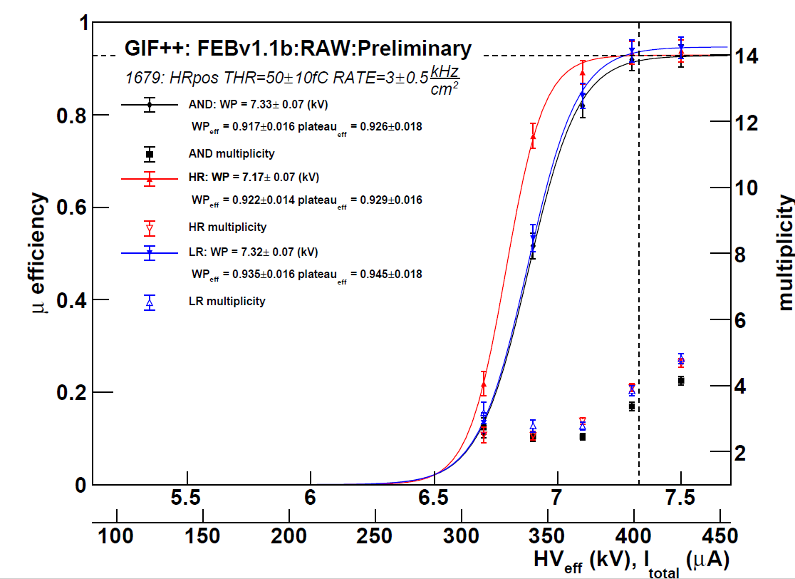
\includegraphics[width=1\textwidth]{uioposter-images/irpc_feb_eff}
    \caption{A capition for iRPC FEB.}
    \label{irpc_feb}
\end{figure}

Bla bla bla ...
    \end{block}

    \vskip-2cm
    \begin{block}{Readout Electronics}
        \vskip-1.5cm
        An extensive Phase-2 upgrade program is also scheduled for CMS Level-1 Trigger~\cite{l1_tdr}. Since RPC is the only Muon detector present in both CMS Barrel and Endcap region, its contribution to CMS Level-1 Trigger upgrade program is important. 

\begin{wrapfigure}{R}{0.6\textwidth}
    \caption{\footnotesize RPC readout and control system for Phase-2.}
    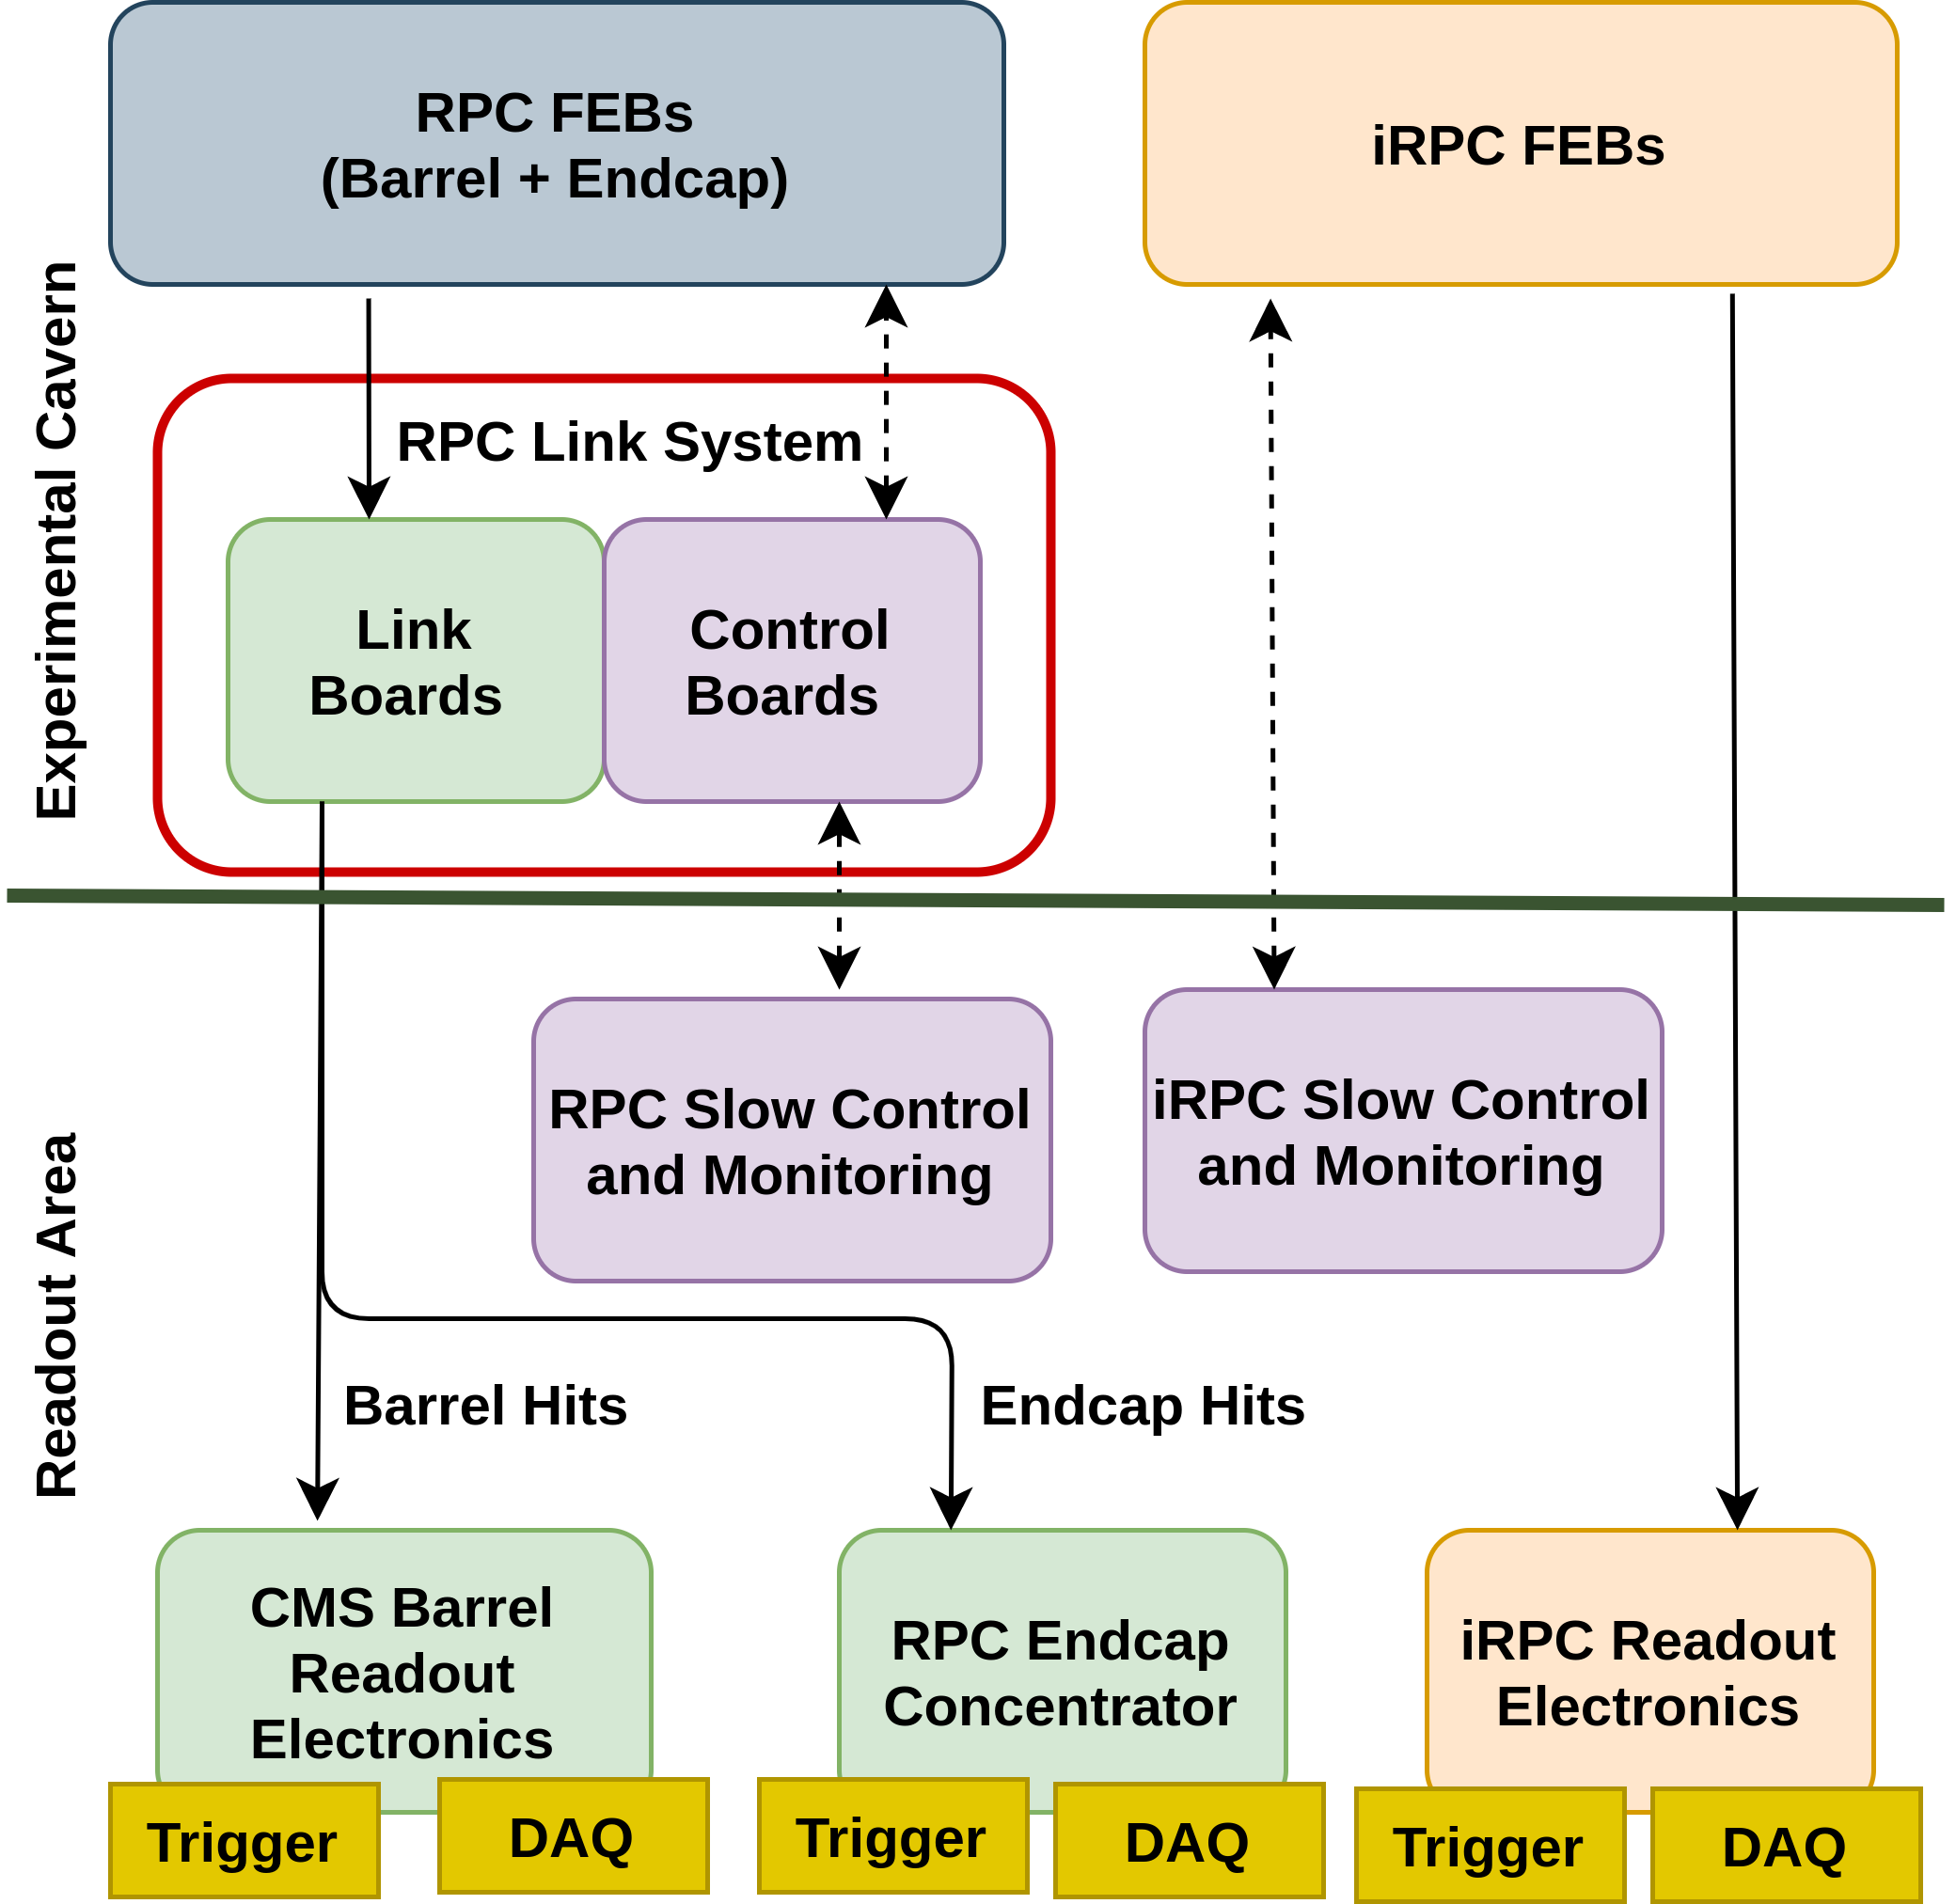
\includegraphics[width=0.6\textwidth]{uioposter-images/rpc_phase2_readout.png}
    \label{rpc_phase2_readout}
\end{wrapfigure}

The readout and control system (also called back-end) of the RPC (Figure 4) system will be redesigned in order to \textbf{(1) include readout and control of new hardware; (2) cope with the requirements of the Level-1 Trigger Phase-2 design; (3) sustain maintainability of the system by replacing obsolete hardware.}

% The readout and control system (also called back-end) of the RPC system will be redesigned in order to:
% \begin{itemize}
%     \item include include readout and control of new hardware;
%     \item cope with the requirements of the CMS Level-1 Trigger Phase-2 design;
%     \item sustain maintenability of the system by replacing obsolete hardware.
% \end{itemize}

The new readout, control and monitoring hardware will be installed in the CMS Services Area, away from CMS radiation, and will follow the CMS specification of common hardware platforms for Phase-2, specifically, Serenity boards~\cite{serenity}, with ATCA form factor. Its links will be composed by Slow Control/Monitoring channels (dashed lines) and readout channels (solid lines). Barrel RPC hits are expected to be distributed to a common CMS Barrel (RPC + DT) hardware, while Endcap and iRPC hits will go to dedicated RPC boards. Those hits will later be distributed to CMS Muon Track Finders and DAQ.

% Different firmwares are expected for the New Link System $\Leftrightarrow$ back-end and iRPC FEB $\Leftrightarrow$ back-end. 
    \end{block}

    \vskip-2cm
    \begin{block}{Demonstrator}
        \vskip-1.5cm
        Bla bla bla...
    \end{block}


\end{column}


% \begin{column}{\textwidth/3 - 2cm}
%     % \begin{alertblock}{How do you make it pop?}
%     %     Use an alert!
%     % \end{alertblock}

%     % \begin{block}{Acknowledgements}
%     %     \lipsum[4]
%     % \end{block}
% \end{column}


\end{columns}
\vskip2cm
\begin{columns}[onlytextwidth]

\begin{column}{\textwidth/2 - 1cm}
    % \vskip-2cm
    \begin{block}{Conclusion}
        \lipsum[75]
    \end{block}
\end{column}

\begin{column}{\textwidth/2 - 1cm}
    % \vskip-2cm
    \begin{block}{References}
        \cite{einstein,einstein2,knuthwebsite,latexcompanion}
        \printbibliography
    \end{block}
\end{column}



\end{columns}


% FOOTNOTE

% \begin{textblock}{1}(0.077, 0.93)
%     % \color{white}
%     % \sffamily
%     % \textbf{TIPP 2021 - International Conference on Technology and Instrumentation in Particle Physics}
    
%     % \printbibliography
    
% \end{textblock}

\end{frame}

\end{document}